\section{Algorithme de filtrage du raisonnement énergétique}
\label{sec:ER_CECSP}
\index{raisonnement énergétique!pour le CECSP}

Le paragraphe ci-dessous décrit l'adaptation du raisonnement
énergétique, introduit par~\cite{RELopez} pour la contrainte cumulative,
et décrit dans le paragraphe~\ref{sec:cumu_propag}. Nous commençons,
dans un premier temps par décrire l'algorithme de vérification de ce
raisonnement, puis nous présenterons les règles d'ajustements qui
peuvent être mises en place pour filtrer les domaines des
variables. Enfin, la dernière partie de ce paragraphe sera consacrée à
la caractérisation des intervalles d'intérêt pour l'algorithme de
vérification et pour les règles d'ajustement.

\subsection{Algorithme de vérification}

\subsubsection{Condition nécessaire d'existence de solution}
Pour décrire l'algorithme de vérification, nous rappelons d'abord
l'idée principale sur laquelle repose le raisonnement énergétique. Le
principe est donc, étant donné un intervalle $[t_1,t_2[$, de calculer
les consommations minimales de ressource des activités dans cette
intervalle et de les comparer à la quantité de ressource disponible
dans ce même intervalle. Si la ressource disponible n'est pas
suffisante pour ordonnancer les consommations minimales de toutes les
activités, une incohérence est détectée.

Dans le cas du \CUSP, la quantité de ressource requise par une
activité pouvait être calculée de manière directe. Ici, ce calcul sera
fait en deux fois: nous calculons d'abord la quantité d'énergie
requise par une activité à l'intérieur de l'intervalle $[t_1,t_2{[}$,
notée $\wb$, puis nous traduisons cette énergie en une quantité de
ressource, notée $\bb$. Ceci nous permettra ensuite de la comparer
avec la ressource disponible dans $[t_1,t_2{[}$.

Formellement ces quantités sont représentées par les expressions
suivantes: 
\begin{align}
  \wb= \min \int_{t_1}^{t_2} f_i(b_i(t))dt & & \text{sous 
\eqref{tw_CECSP}-\eqref{nrj_CECSP}}\\
  \bb= \min \int_{t_1}^{t_2} b_i(t)dt & & \text{sous 
\eqref{tw_CECSP}-\eqref{nrj_CECSP}} \label{eq:minConso}
\end{align}

Comme pour le cas du \CUSP, la fonction de marge, notée $SL(t_1,t_2)$,
permet de mesurer l'écart entre la quantité de ressource disponible et
les consommations minimales de toutes les tâches dans l'intervalle
${[}t_1,t_2{]}$. Cette fonction est définie de la manière suivante:
\[ SL(t_1,t_2)=B(t_2-t_1)-\sum\limits_{i \in A} \bb \]

Et ceci nous permet d'énoncer la condition nécessaire d'existence
d'une solution qui est à la base de l'algorithme de vérification du
raisonnement énergétique:

\begin{theo}
  \label{th:ER_CECSP}
  Soit $\I$ une instance du \CECSP. S'il existe $t_1 < t_2 \in
  \mathbb{R}^2$ tel que $SL(t_1,t_2) <0$ alors $\I$ ne peut pas avoir
  de solution.
\end{theo}

\begin{proof}
Par l'absurde, supposons qu'il existe $t_1 < t_2 \in \mathbb{R}^2$ tel
que $SL(t_1,t_2) > 0$ et que l'instance $\I$ soit satisfiable. Par
définition, $\bb$ est la quantité de ressource minimale que doit
consommer l'activité $i$ dans l'intervalle $[t_1,t_2{[}$. 

Donc, dans toute solution réalisable, nous avons: 
\begin{align*}
 & \int_{t_1}^{t_2} b_i(t)dt \ge \bb\\
\Rightarrow  & \sum_{i \in \A} \int_{t_1}^{t_2} b_i(t)dt \ge \sum_{i
               \in \A}  \bb > R(t_2-t_1)
\end{align*}
Et ceci contredit le fait que $\sum_{i \in \A} b_i(t) \le
R(t_2-t_1)$. 
\end{proof}

Dans un premier temps, nous allons nous intéressé au calcul de $\wb$,
le calcul de $\bb$ sera détaillé dans un second temps. 


\subsubsection{{\'E}nergie minimale dans un intervalle}

Pour calculer $\wb$, nous analysons les différentes configurations de
la consommation minimale d'une tâche. Remarquons que les
configurations conduisant à une consommation minimale dans
l'intervalle $[t_1,t_2{[}$ sont celles où l'activité est ordonnancée à
$\bmax$ à l'intérieur de cet intervalle. Ces configurations, décrites
dans la figure~\ref{fig:conso_CECSP}, peuvent être regroupée en trois
catégories:
\begin{itemize}
\item l'activité est {\it calée à
gauche} (figure~\ref{fig:conso_CECSPa}, \ref{fig:conso_CECSPb},
\ref{fig:conso_CECSPd} et \ref{fig:conso_CECSPg}): l'activité démarre
à $\ES$ et est ordonnancée à $\bmax$ pendant l'intervalle
$[\ES,t_1{[}$;
\item l'activité est {\it calée à
droite} (figure~\ref{fig:conso_CECSPb}, \ref{fig:conso_CECSPc},
\ref{fig:conso_CECSPf} et \ref{fig:conso_CECSPi}): l'activité finit à
$\LE$ et est ordonnancée à $\bmax$ pendant l'intervalle $[t_2,\LE{[}$;
\item l'activité est {\it centrée} (figure~\ref{fig:conso_CECSPe} et
\ref{fig:conso_CECSPh}): l'activité occupe tout l'intervalle
$[t_1,t_2[$, soit en étant ordonnancée à $\bmax$ pendant l'intervalle
$[\ES,t_1{[} \cup [t_2,\LE{[}$, soit en étant ordonnancée à $\bmin$
durant tout l'intervalle $[t_1,t_2{[}$.
\end{itemize}
En effet, lorsque l'activité est ordonnancée à $\bmax$ pendant
l'intervalle $[\ES,t_1{[} \cup [t_2,\LE{[}$, il peut arriver que la
quantité d'énergie restant à apporter à l'activité durant l'intervalle
$[t_1,t_2[$ ne soit pas suffisante pour assurer la satisfaction de la
contrainte de consommation minimale~\eqref{req_CECSP}. Le cas où
l'activité est ordonnancée à $\bmin$ durant tout l'intervalle
$[t_1,t_2{[}$ doit donc être considéré.

\begin{figure}[!htb]  
\centering
\subcaptionbox{\label{fig:conso_CECSPa}}[0.3\linewidth]{
  \begin{tikzpicture}
    [xscale=0.37,yscale=0.3]
    \node[] (O) at (0,0) {};
    \node[label={[shift={(-0.4,-0.4)}]$\bmin$}] (bmin) at (0,1) {};
    \node[label={[shift={(-0.4,-0.4)}]$\bmax$}] (bmax) at (0,4) {};
    \node (t1) at (6,0) {}; 
    \node[label={[shift={(0,-0.8)}]$\ES$}] (ri) at (1,0) {};
    \node (t2) at (7,0) {};

    \draw[->] (O.center) -- (8,0)node[below] {$t$};
    \draw (O.south) -- (bmax.north);
    \draw (bmin.center) -- (8,1);
    \draw (bmax.center) -- (8,4);
    \draw(ri.south) -- (ri.center);
    \draw[fill=white] (ri.center) rectangle (5,4);
    \draw[pattern=north west lines] (ri.center) rectangle (5,4);
    \draw[thick] (t1.south) -- (6,4.1) node[above] {$t_1$};
    \draw[thick] (t2.south) -- (7,4.1) node[above] {$t_2$};
  \end{tikzpicture}}
\hfill
\subcaptionbox{\label{fig:conso_CECSPb}}[0.3\linewidth]{
  \begin{tikzpicture}
    [xscale=0.37,yscale=0.3]
    \node[] (O) at (0,0) {};
    \node[label={[shift={(-0.4,-0.4)}]$\bmin$}] (bmin) at (0,1) {};
    \node[label={[shift={(-0.4,-0.4)}]$\bmax$}] (bmax) at (0,4) {};
    \node (t1) at (1,0) {}; 
    \node[label={[shift={(0,-0.8)}]$\ES$}] (ri) at (2,0) {};
    \node (t2) at (7,0) {};
    \node[label={[shift={(0,-0.8)}]$\LE$}] (di) at (6,0) {};

    \draw[->] (O.center) -- (8,0)node[below] {$t$};
    \draw (O.south) -- (bmax.north);
    \draw (bmin.center) -- (8,1);
    \draw (bmax.center) -- (8,4);
    \draw(ri.south) -- (ri.center);
    \draw(di.south) -- (di.center);
    \draw[fill=white] (2.5,0) rectangle (5.5,4);
    \draw[pattern=north west lines] (2.5,0) rectangle (5.5,4);
    \draw[thick] (t1.south) -- (1,4.1) node[above] {$t_1$};
    \draw[thick] (t2.south) -- (7,4.1) node[above] {$t_2$};
  \end{tikzpicture}}
\hfill
\subcaptionbox{\label{fig:conso_CECSPc}}[0.3\linewidth]{
  \begin{tikzpicture}
    [xscale=0.37,yscale=0.3]
    \node[] (O) at (0,0) {};
    \node[label={[shift={(-0.4,-0.4)}]$\bmin$}] (bmin) at (0,1) {};
    \node[label={[shift={(-0.4,-0.4)}]$\bmax$}] (bmax) at (0,4) {};
    \node (t1) at (0.5,0) {};
    \node (t2) at (1.5,0) {};
    \node[label={[shift={(0,-0.8)}]$\LE$}] (di) at (7,0) {};
    
    \draw[->] (O.center) -- (8,0)node[below] {$t$};
    \draw (O.south) -- (bmax.north);
    \draw (bmin.center) -- (8,1);
    \draw (bmax.center) -- (8,4);
    \draw[fill=white] (3,0) rectangle (7,4);
    \draw[pattern=north west lines] (3,0) rectangle (7,4);
    \draw(di.south) -- (di.center);
    \draw[thick] (t1.south) -- (0.5,4.1) node[above] {$t_1$};
    \draw[thick] (t2.south) -- (1.5,4.1) node[above] {$t_2$};
  \end{tikzpicture}}


\subcaptionbox{\label{fig:conso_CECSPd}}[0.3\linewidth]{
\begin{tikzpicture}
  [xscale=0.37,yscale=0.3]
    \node[] (O) at (0,0) {};
    \node[label={[shift={(-0.4,-0.4)}]$\bmin$}] (bmin) at (0,1) {};
    \node[label={[shift={(-0.4,-0.4)}]$\bmax$}] (bmax) at (0,4) {};
    \node (t1) at (4,0) {};
    \node (t2) at (7,0) {};
    \node[label={[shift={(0,-0.8)}]$\LE$}] (di) at (6,0) {};
    \node[label={[shift={(0,-0.8)}]$\ES$}] (ri) at (1,0) {};
    
    \draw[->] (O.center) -- (8,0)node[below] {$t$};
    \draw (O.south) -- (bmax.north);
    \draw (bmin.center) -- (8,1);
    \draw (bmax.center) -- (8,4);
    \draw[fill=white] (ri.center) rectangle (4,4);
    \draw[pattern=north west lines] (ri.center) rectangle (4,4);
    \draw[fill=white] (t1.center) rectangle (5,1.5);
    \draw[pattern=north west lines] (t1.center) rectangle (5,1.5);
    \draw(di.south) -- (di.center);
    \draw(ri.south) -- (ri.center);
    \draw[thick] (t1.south) -- (4,4.1) node[above] {$t_1$};
    \draw[thick] (t2.south) -- (7,4.1) node[above] {$t_2$};
  \end{tikzpicture}}
\hfill
\subcaptionbox{\label{fig:conso_CECSPe}}[0.3\linewidth]{
\begin{tikzpicture}
 [xscale=0.37,yscale=0.3]
 \node[] (O) at (0,0) {};
 \node[label={[shift={(-0.4,-0.4)}]$\bmin$}] (bmin) at (0,1) {};
 \node[label={[shift={(-0.4,-0.4)}]$\bmax$}] (bmax) at (0,4) {};
 \node (t1) at (2.5,0) {}; 
 \node[label={[shift={(0,-0.8)}]$\ES$}] (ri) at (1.5,0) {};
 \node (t2) at (6,0) {};
 \node[label={[shift={(0,-0.8)}]$\LE$}] (di) at (7,0) {};
 
  \draw[->] (O.center) -- (8,0)node[below] {$t$};
  \draw (O.south) -- (bmax.north);
  \draw (bmin.center) -- (8,1);
  \draw (bmax.center) -- (8,4);
  \draw(ri.south) -- (ri.center);
  \draw(di.south) -- (di.center);
  \draw[fill=white] (2.5,0) rectangle (1.5,4);
  \draw[pattern=north west lines] (2.5,0) rectangle (1.5,4);
  \draw[fill=white] (2.5,0) rectangle (6,2);
  \draw[pattern=north west lines] (2.5,0) rectangle (6,2);
  \draw[fill=white] (6,0) rectangle (7,4);
  \draw[pattern=north west lines] (6,0) rectangle (7,4);
  \draw[thick] (t1.south) -- (2.5,4.1) node[above] {$t_1$};
  \draw[thick] (t2.south) -- (6,4.1) node[above] {$t_2$};
 \end{tikzpicture}}
\hfill
\subcaptionbox{\label{fig:conso_CECSPf}}[0.3\linewidth]{
  \begin{tikzpicture}
 [xscale=0.37,yscale=0.3]
 \node[] (O) at (0,0) {};
 \node[label={[shift={(-0.4,-0.4)}]$\bmin$}] (bmin) at (0,1) {};
 \node[label={[shift={(-0.4,-0.4)}]$\bmax$}] (bmax) at (0,4) {};
 \node[label={[shift={(0,-0.8)}]$\LE$}] (di) at (7,0) {};
 \node (t1) at (1,0) {}; 
 \node[label={[shift={(0,-0.8)}]$\ES$}] (ri) at (2.5,0) {};
 \node (t2) at (4,0) {};
 
 \draw[->] (O.center) -- (8,0)node[below] {$t$};
 \draw (O.south) -- (bmax.north);
 \draw (bmin.center) -- (8,1);
 \draw (bmax.center) -- (8,4);
 \draw(di.south) -- (di.center);
 \draw(ri.south) -- (ri.center);
 \draw[fill=white] (t2.center) rectangle (7,4);
 \draw[pattern=north west lines] (t2.center) rectangle (7,4);
 \draw[fill=white] (t2.center) rectangle (3.2,2);
 \draw[pattern=north west lines] (t2.center) rectangle (3.2,2);
 \draw[thick] (t1.south) -- (1,4.1) node[above] {$t_1$};
 \draw[thick] (t2.south) -- (4,4.1) node[above] {$t_2$};
 \end{tikzpicture}}



\subcaptionbox{\label{fig:conso_CECSPg}}[0.3\linewidth]{
  \begin{tikzpicture}
  [xscale=0.37,yscale=0.3]
    \node[] (O) at (0,0) {};
    \node[label={[shift={(-0.4,-0.4)}]$\bmin$}] (bmin) at (0,1) {};
    \node[label={[shift={(-0.4,-0.4)}]$\bmax$}] (bmax) at (0,4) {};
    \node (t1) at (3,0) {};
    \node (t2) at (5,0) {};
    \node[label={[shift={(0,-0.8)}]$\LE$}] (di) at (7,0) {};
    \node[label={[shift={(0,-0.8)}]$\ES$}] (ri) at (1,0) {};
    
    \draw[->] (O.center) -- (8,0)node[below] {$t$};
    \draw (O.south) -- (bmax.north);
    \draw (bmin.center) -- (8,1);
    \draw (bmax.center) -- (8,4);
    \draw[fill=white] (t1.center) rectangle (1,4);
    \draw[pattern=north west lines] (t1.center) rectangle (1,4);
    \draw[fill=white] (t1.center) rectangle (3.7,1);
    \draw[pattern=north west lines] (t1.center) rectangle (3.7,1);
    \draw(di.south) -- (di.center);
    \draw(ri.south) -- (ri.center);
    \draw[thick] (t1.south) -- (3,4.1) node[above] {$t_1$};
    \draw[thick] (t2.south) -- (5,4.1) node[above] {$t_2$};
  \end{tikzpicture}}
\hfill
\subcaptionbox{\label{fig:conso_CECSPh}}[0.3\linewidth]{
  \begin{tikzpicture}
  [xscale=0.37,yscale=0.3]
   \node[] (O) at (0,0) {};
    \node[label={[shift={(-0.4,-0.4)}]$\bmin$}] (bmin) at (0,1) {};
    \node[label={[shift={(-0.4,-0.4)}]$\bmax$}] (bmax) at (0,4) {};
    \node (t1) at (2.5,0) {}; 
    \node[label={[shift={(0,-0.8)}]$\ES$}] (ri) at (1.5,0) {};
    \node (t2) at (6,0) {};
    \node[label={[shift={(0,-0.8)}]$\LE$}] (di) at (7,0) {};

    \draw[->] (O.center) -- (8,0)node[below] {$t$};
    \draw (O.south) -- (bmax.north);
    \draw (bmin.center) -- (8,1);
    \draw (bmax.center) -- (8,4);
    \draw(ri.south) -- (ri.center);
    \draw(di.south) -- (di.center);
    \draw[fill=white] (2.5,0) rectangle (2,2.7);
    \draw[pattern=north west lines] (2.5,0) rectangle (2,2.7);
    \draw[fill=white] (2.5,0) rectangle (6,1);
    \draw[pattern=north west lines] (2.5,0) rectangle (6,1);
    \draw[fill=white] (6,0) rectangle (7,4);
    \draw[pattern=north west lines] (6,0) rectangle (7,3);
    \draw[thick] (t1.south) -- (2.5,4.1) node[above] {$t_1$};
    \draw[thick] (t2.south) -- (6,4.1) node[above] {$t_2$};
  \end{tikzpicture}}
\hfill
\subcaptionbox{\label{fig:conso_CECSPi}}[0.3\linewidth]{
\begin{tikzpicture}
 [xscale=0.37,yscale=0.3]
 \node[] (O) at (0,0) {};
 \node[label={[shift={(-0.4,-0.4)}]$\bmin$}] (bmin) at (0,1) {};
 \node[label={[shift={(-0.4,-0.4)}]$\bmax$}] (bmax) at (0,4) {};
 \node[label={[shift={(0,-0.8)}]$\LE$}] (di) at (7,0) {};
 \node (t1) at (2.5,0) {}; 
 \node (t2) at (4,0) {};
 \node[label={[shift={(0,-0.8)}]$\ES$}] (ri) at (1,0) {};
 
 \draw[->] (O.center) -- (8,0)node[below] {$t$};
 \draw (O.south) -- (bmax.north);
 \draw (bmin.center) -- (8,1);
 \draw (bmax.center) -- (8,4);
 \draw(di.south) -- (di.center);
 \draw(ri.south) -- (ri.center);
 \draw[fill=white] (t2.center) rectangle (7,4);
 \draw[pattern=north west lines] (t2.center) rectangle (7,4);
 \draw[fill=white] (t2.center) rectangle (3.2,1);
 \draw[pattern=north west lines] (t2.center) rectangle (3.2,1);
 \draw[thick] (t1.south) -- (2.5,4.1) node[above] {$t_1$};
 \draw[thick] (t2.south) -- (4,4.1) node[above] {$t_2$}; 
 \end{tikzpicture}}
\caption{Les différentes configurations menant à une consommation minimale}
\label{fig:conso_CECSP}
\end{figure}
	
Il est facile de calculer l'expression de la consommation minimale
d'énergie dans un intervalle pour une fonction $f_i$ croissante. En
effet, les différentes configurations possibles étant toujours celle
où la tâche est exécutée à son rendement maximum en dehors de
l'intervalle ${[}t_1,t_2{[}$, il suffit de retrancher à $W_i$
l'énergie produite par l'exécution de la tâche en dehors de
${[}t_1,t_2{]}$. Il existe une exception à cette règle, produite par
la contrainte du rendement minimal, mais ce cas est facilement traiter
puisque l'énergie minimale correspond alors à la configuration où la
tâche est exécutée à son rendement minimal durant ${[}t_1,t_2{[}$. 

Pour donner l'expression mathématique de $\wb$ , nous introduisons
trois notations. $\wbLS$ (respectivement $\wbRS$ et $\wbCS$)
correspond à la quantité d'énergie apportée à l'activité $i$ dans
l'intervalle $[t_1,t_2[$ quand l'activité est calée à gauche
(respectivement calée à droite et centrée). Formellement, ces trois
quantités peuvent être exprimer de la manière suivante:
\begin{align}
\wbLS&= \max\left(0\, ,\, W_i- f_i(\bmax)\max(0,t_1 -
\ES)\right) \label{eq:LSnrj_CECSP}\\
\wbRS&= \max\left(0\, ,\, W_i- f_i(\bmax)\max(0,
\LE-t_2)\right)\label{eq:RSnrj_CECSP}\\
\wbCS&=\max\left( f_i(\bmin) * (t_2-t_1)\, ,\, W_i - f_i(\bmax)\max(0,
d_i - r_ i - t_2 + t_1) \right)\label{eq:CSnrj_CECSP}
\end{align}
Alors, l'expression de l'énergie minimale est le minimum de ces trois
quantités, i.e.
\begin{equation}
\wb=\min\left(\, \wbLS\, ,\,\wbRS\, ,\,\wbCS \, \right)
\end{equation} 

Nous allons maintenant utiliser l'expression de $\wb$ et la fonction
$f_i$ pour calculer $\bb$.

\subsubsection{Consommation minimale de la ressource}
	
Pour calculer l'expression de $\bb$, nous allons utiliser les
propriétés de la fonction $f_i$. En effet, une fois que nous avons
calculer $\wb$, nous voulons savoir quelle est la quantité minimale de
ressource que nous devons fournir à la tâche pour obtenir cette
quantité d'énergie dans l'intervalle ${[}t_1,t_2{[}$. Dans le cas où
la fonction $f_i$ est l'identité, nous avons que: $\bb=\wb$. Dans les
deux autres cas, i.e. $f_i$ est affine et $f_i$ est concave et affine
par morceaux, soit $I=[t_1,t_2[ \cap [\ES,\LE{[}$, alors trouver $\bb$
revient à résoudre le programme suivant:
\begin{align}
  \text{minimiser }   & \int_{I} b_i(t)dt \label{eq:conv_obj} \\
  \text{sous } & \int_{I} f_i(b_i(t))dt \ge \wb \label{eq:conv_nrj}\\
                     & \bmin \le b_i(t) \le \bmax \label{eq:conv_min}
\end{align}
En effet, l'objectif de ce programme est de minimiser la quantité de
ressource consommée dans l'intervalle $[t_1,t_2[$
(équation~\eqref{eq:conv_obj}), tout en s'assurant que l'énergie
requise, i.e. $\wb$, est bien apportée à l'activité
(équation~\eqref{eq:conv_nrj}). 

Nous utilisons ensuite le lemme~\ref{lemmaEn} pour simplifier ce
programme. En effet, le lemme affirme que, si $f_i$ est affine ou
concave et affine par morceaux, alors si une solution optimale
$b_i(t)$ pour le programme ci-dessus, cette solution peut être
transformée en une autre solution optimale vérifiant la propriété que
$b_i(t)$ soit constante et inférieure ou égale à
$\frac{\int_{I}b_i(t)dt}{|I|}$. Nous noterons $b_i$ cette
constante. Le programme simplifié s'écrit de la manière suivante:
\begin{align}
  \text{minimiser }   & b_i|I| \label{eq:convSimp_obj} \\
  \text{sous } & f_i(b_i)|I| \ge \wb \label{eq:convSimp_nrj}\\
                     &\bmin \le  b_i \le \bmax \label{eq:convSimp_nrj}
\end{align}


Ce programme peut être réécrit de la façon suivante: 
\[ b_i=\min\left( b \in [\bmin,\bmax]\ |\ f_i(b) \ge
    \frac{\wb}{|I|}\right)
\]

Nous pouvons remarquer que, si l'on suppose que $f_i(\bmax) (\LE - \ES
) \ge W_i$, nous sommes sûrs que la solution optimale vérifie $b_i \le
\bmax$. En effet, ceci est dû au fait qu'exécuter l'activité à une
faible consommation de ressource a un meilleur rendement que son
exécution à un rendement plus élevé, i.e. la fonction
$\frac{f_i(b_i(t))}{b_i(t)}$ est décroissante. 

De ce fait, seule la borne inférieure sur $b_i$, $\bmin$, doit être
considérée. Or, pour apporter l'énergie $\wb$ à l'activité dans
l'intervalle $I$, sa consommation $b_i$ doit vérifiée $f_i(b_i) \ge
\frac{\wb}{|I|}$ et donc $b_i \ge
f_i^{-1}\left(\frac{\wb}{|I|}\right)$. En couplant cette contrainte
avec la contrainte de consommation minimale, nous obtenons, si $\bmin
\neq 0$:
\[
 b_i= \max\left(\, \bmin \, ,\, 
    f_i^{-1}\left(\frac{\wb}{|I|}\right)\, \right)
\]
Et si $\bmin = 0$, nous avons:
\[
 b_i=  f_i^{-1}\left(\frac{\wb}{|I|}\right)
\]
Nous allons maintenant donner l'expression de $\bb$  en fonction des
coefficients $a_{ip}$  et $c_{ip}$ de la fonction $f_i$. Pour
simplifier la compréhension, nous commençons par détailler cette
expression dans le cas où $f_i$ est affine puis nous la généraliserons
dans le cas où $f_i$ est concave et affine par morceaux. 

\paragraph{Fonctions affines}

Dans ce paragraphe, nous allons décrire l'expression de $\bb$ dans le
cas où la fonction $f_i$ est affine, i.e. de la forme $a_ib+c_i$. Dans
ce cas-là, nous avons:  
\[f_i^{-1}\left( \frac{\wb}{|I|}\right)= \frac{ \wb- c_i|I|}{a_i|I|}
\]
Et donc, si $\bmin\neq 0$: 
\begin{equation}
\bb= \max\left(b_i^{min} \frac{\wb}{f_i(b_i^{min})} \, ,\,  
  \frac{1}{a_i}\left(\wb-|I|c_{i})\right)\right)
\end{equation}
Et si $\bmin=0$: 
\[
\bb=  \frac{1}{a_i}\left(\wb-|I|c_{i})\right)
\]
Notons que, le premier cas correspond au cas où l'intervalle $I$ est
suffisamment grand pour ordonnancer l'activité $i$ à $\bmin$ et lui
apporter l'énergie requise, i.e. $\wb$. En effet, comme ordonnancer
$i$ à $\bmin$ a la meilleur rendement, si l'on peut, i.e. l'intervalle
est assez grand, c'est cette valeur que l'on va choisir pour
$b_i$. Si, au contraire, l'intervalle n'est pas suffisamment grand,
c'est $f_i^{-1}(\wb/|I|) \times |I|$ que l'on va choisir. Ceci est
détaillé dans l'exemple~\ref{ex:convLin_CECSP}.

\begin{ex}
\label{ex:convLin_CECSP}

\end{ex}

Ce raisonnement peut être étendu dans le cas où $f_i$ est concave et
affine par morceaux. 

\paragraph{Fonctions concave et affine par morceaux}

Dans le cas des fonctions concaves et affines par morceaux, le
raisonnement décrit au paragraphe précédent peut être généralisé. En
effet, comme dans le cas des fonctions affines, la fonction de
rendement, $f_i(b_i(t))/b_i(t)$, est décroissante. Donc, il est
toujours préférable d'exécuter l'activité avec une consommation de
ressource aussi basse que possible. La condition selon laquelle on
peut ou non exécuter l'activité $i$ avec une consommation $b_i$ dépend
donc de la taille de l'intervalle $I$. 

Si $\bmin\neq 0$ et si l'intervalle est suffisamment grand, on va donc
exécuter l'activité à $\bmin$. Sinon, et si l'intervalle est
suffisamment grand, nous essayons d'exécuter l'activité avec une
consommation $b_i \in ]\bmin,x_2^i]$, etc. Dans le cas où $\bmin \neq
0$, l'expression de $\bb$ est formalisée ci-dessous:
\[f_i^{-1}\left(\frac{\wb}{|I|}\right)=\left\{
\begin{aligned}
\bmin & \qquad & \text{si } |I| \ge \frac{\wb}{f_i(\bmin)}\\
\frac{\wb -c_{i1}|I|}{a_{i1}|I|} & \qquad & \text{si } \frac{\wb}{f_i(\bmin)}
> |I| > \frac{\wb}{f_i(x^i_2)} \\
\frac{\wb -c_{i2}|I|}{a_{i2}|I|} & \qquad & \text{si }  \frac{\wb}{f_i(x^i_2)}
\ge |I| > \frac{\wb}{f_i(x^i_3)}\\
 & \qquad \vdots& \\
\frac{\wb -c_{iP_i}|I|}{a_{iP_i}|I|} & \qquad & \text{si }  \frac{\wb}{f_i(x^i_{P_i}}
\ge |I| > \frac{\wb}{f_i(\bmax)}\end{aligned}
\right.
\]
Et ceci, nous donne l'expression de $\bb$ suivante:
\begin{equation}
\bb= 
  \max \left\{b_i^{min} \frac{\wb}{f_i(b_i^{min})},
  \max_{ p \in \P_i} \left(\frac{1}{a_{ip}}(\wb-|I|c_{ip})\right)\right\}
\end{equation}
Dans le cas où $\bmin=0$, nous avons: 
\[
\bb= 
  \max_{ p \in \P_i} \left(\frac{1}{a_{ip}}(\wb-|I|c_{ip})\right)
\]
Un exemple du calcul de $\bb$ dans le cas d'une fonction $f_i$ concave
et linéaire par morceaux est décrit dans
l'exemple~\ref{ex:convPWL_CECSP}.

\begin{ex}
\label{ex:convPWL_CECSP}

\end{ex}

\subsection{Les ajustements de borne}
\label{sec:adjustment_tw}
 
Dans ce paragraphe nous décrivons les ajustements qui peuvent être
faits sur les fenêtre de temps des activités. Tout d'abord, nous
introduisons les notations suivantes: $\bbLS$ (respectivement $\bbRS$
et $\bbCS$) correspond à la quantité de ressource consommée par
l'activité $i$ dans l'intervalle $[t_1,t_2[$ quand l'activité est
calée à gauche (respectivement calée à droite et
centrée). Formellement, ces trois quantités peuvent être exprimer de
la manière suivante:
\begin{align}
\bbLS&=   \max \left\{b_i^{min} \frac{\wbLS}{f_i(b_i^{min})},
  \max_{ p \in \P_i} \left(\frac{1}{a_{ip}}(\wbLS-|I|c_{ip})\right)\right\}\\
\bbRS&=   \max \left\{b_i^{min} \frac{\wbRS}{f_i(b_i^{min})},
  \max_{ p \in \P_i} \left(\frac{1}{a_{ip}}(\wbRS-|I|c_{ip})\right)\right\}\\
\bbCS&=  \max \left\{b_i^{min} \frac{\wbCS}{f_i(b_i^{min})},
  \max_{ p \in \P_i} \left(\frac{1}{a_{ip}}(\wbCS-|I|c_{ip})\right)\right\}
\end{align}

Nous allons décrire deux règles d'ajustements pour les fenêtres du
temps du \CECSP. La première permet d'ajuster $\LS$ et la seconde
$\ES$ et nous avons des ajustements symétriques pour $\EE$ et $\LE$. 

Pour les premier ajustements décrits, nous allons essayer de faire
démarrer l'activité après $t_1$et si la quantité de ressource
disponible n’est pas suffisante pour ordonnancer les consommations
minimales de toutes les activités – excepté celle de l’activité i qui
est remplacée par $\bbRS$ – alors, nous pouvons déduire que l’activité
doit commencer avant $t_1$.

\begin{reg}
\label{reg:ajust_CECSP}
S’il existe un intervalle $[t_1 , t_2 [$ avec $t_1 > \ES$ et une
activité $i$ pour lesquels:
\[ \sum_{\substack{j \in \A\\ j\neq i}} \bb[j] + \bbRS > R(t_2-t_1)
\]
alors, on a:
\[ \LS \le t_1 - \frac{1}{\bmax}\left(\sum_{\substack{j \in \A\\ j\neq i}} \bb[j] + \bbRS - R(t_2-t_1)\right)
\]
\end{reg}

\begin{proof}
Soit $i$ et $[t_1,t_2[$ vérifiant la condition de la
règle~\ref{reg:ajust_CECSP}. Supposons que l'activité $i$ démarre à
$t_1$. 

La consommation minimale de $i$ dans $[t_1,t_2[$ est donc $\bbRS$. On
a donc que $\sum_{\substack{j \in \A\\ j\neq i}} \bb[j] + \bbRS $ est
la consommation minimale de toutes les activités dans $[t_1,t_2[$
quand l'activité $i$ commence à $t_1$. Donc, si cette quantité est
plus grande que la quantité de ressource disponible dans l'intervalle
$[t_1,t_2[$, i.e. $R(t_2-t_1)$, on obtient une contradiction avec le
fait que l'instance soit réalisable et $i$ doit commencer avant
$t_1$. 

Pour calculer la nouvelle date de début au plus tard de $i$,
remarquons que la quantité de ressource devant être consommée avant
$t_1$ est d'au moins $\sum_{\substack{j \in \A\\ j\neq i}} \bb[j] +
\bbRS - R(t_2-t_1)$, i.e. ce qui ne ``rentrait'' pas dans
$[t_1,t_2[$. Comme nous cherchons une borne supérieure sur la date de
début de $i$, nous cherchons donc à ordonnancer cette partie de
l'activité le plus rapidement possible. 

Le temps minimal requis pour ordonnancer cette
consommation étant obtenu en exécutant l'activité à $\bmax$, nous
obtenons comme borne supérieure sur la date de début de $i$:
$1/\bmax \times \left(\sum_{\substack{j \in \A\\ j\neq
i}} \bb[j] + \bbRS - R(t_2-t_1)\right)$
\end{proof}

De manière similaire, nous avons les ajustements suivants sur la date
de début au plus tôt d'une activité. 
\begin{reg}
\label{reg:ajustRi_CECSP}
S'il existe un intervalle $[t_1,t_2[$ avec $ t_2 > \LE$ et une
activité $i$ telle que $\bmin \neq 0$ pour lesquels:
  \[ \sum_{\substack{j \in \A \\ j \neq i}} \bb[j] +
    \min(\bbCS,\bbLS) > R (t_2-t_1)\] 
  alors
  \[ \ES \ge t_2 - \frac{1}{\bmin} \left(R (t_2-t_1) -\sum_{\substack{j
\in \A \\ j \neq i}} \bb[j] \right) \]
\end{reg}

\begin{proof}
Soit $i$ et $[t_1,t_2[$ vérifiant la condition de la
règle~\ref{reg:ajust_CECSP}. Nous allons décider si $i$ peut commencer
avant $t_1$. Les configurations où l'activité $i$ démarre avant $t_1$
et consomme le moins de ressource possible dans $[t_1,t_2[$ sont les
configurations où $i$ est soit calée à gauche, soit centrée.

La consommation minimale de $i$ dans l'intervalle $[t_1,t_2[$ quand
$i$ commence avant $t_1$ est donc $\min( \bbLS, \bbCS)$. On a donc que
$\sum_{\substack{j \in \A\\ j\neq i}} \bb[j] + \min( \bbLS, \bbCS) $
est la consommation minimale de toutes les activités dans $[t_1,t_2[$
quand l'activité $i$ commence avant $t_1$. Donc, si cette quantité est
plus grande que la quantité de ressource disponible dans l'intervalle
$[t_1,t_2[$, i.e. $R(t_2-t_1)$, on obtient une contradiction avec le
fait que l'instance soit réalisable et $i$ doit commencer après $t_1$.

Pour calculer la nouvelle date de début au plus tard de $i$,
remarquons que la quantité de ressource disponible dans $[t_1,t_2[$
pour exécuter $i$ est de $R(t_2-t_1) -\sum_{\substack{j \in \A\\
j\neq i}} \bb[j]$. Comme nous cherchons une borne inférieure sur la date de
début de $i$, nous cherchons donc à ordonnancer cette partie de
l'activité le moins rapidement possible. 

Le temps maximal requis pour ordonnancer cette consommation étant
obtenu en exécutant l'activité à $\bmin$, et, comme $\bmin \neq 0$,
l'activité ne peut être préemptée, nous savons que l'activité doit
être en cours à $t_2$. Nous obtenons alors comme borne inférieure sur
la date de début de $i$:
$t_2 - 1/\bmin \left(R (t_2-t_1) -\sum_{\substack{j
\in \A \\ j \neq i}} \bb[j] \right) $
\end{proof}

\begin{ex}
 Considérons l'instance à $3$ activités et avec $R=5$ suivante:

  \begin{center}
    \begin{tabular}{|P{1cm}|P{1cm}P{1cm}P{1cm}P{1cm}P{1cm}P{2cm}|} 
      \hline 
      act. & \ES & \LE & W_i & \bmin& \bmax & f_i(b_i(t))\\ 
      \hline 
      1 & 0 & 6 & 28 & 1 & 5 & 2b_i(t)+1\\ 
      2 & 2 & 6 & 32 & 2 & 5 & b_i(t)+5\\ 
      3 & 2 & 5 & 6 & 2 & 2 & b_i(t)\\ 
      \hline
    \end{tabular}
  \end{center}
Une solution réalisable est décrit par la figure~\ref{exSol}.
\begin{figure}[!htb]
  \begin{center} 
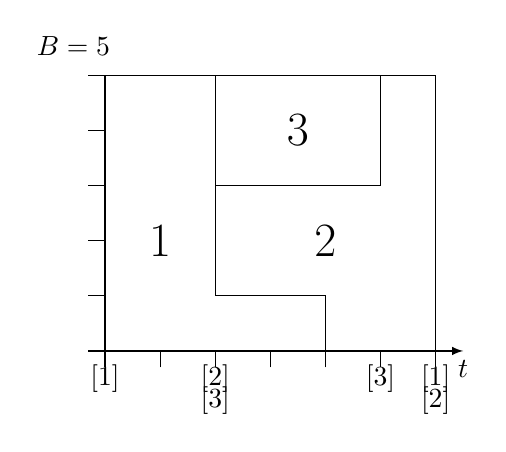
\begin{tikzpicture}
[scale=0.7]
\node (O) at (0,0) {};
\node (2) at (4,2) {\LARGE $2$};
\node (1) at (1,2) {\LARGE $1$};
\node (3) at (3.5,4) {\LARGE $3$};
\node[label={[shift={(-0.4,0)}]$B=5$}] (B) at (0,5) {};


\node (r1) at (0,-0.5) {$\ES[1]$}; 
\node (r2) at (2,-0.5) {$\ES[2]$};
\node (r3) at (2,-0.9) {$\ES[3]$};
\node (d1) at (6,-0.5) {$\LE[1]$};
\node (d2) at (6,-0.9) {$\LE[2]$};
\node (d3) at (5,-0.5) {$\LE[3]$};


\draw[->,>=latex] (6,0) -- (6.5,0) node[below] {$t$};

%\draw (0,0) rectangle (6,5);
\draw (4,0) -- (6,0) -- (6,5) -- (5,5);

   \draw (2,5) -- (2,1) -- (4,1) -- (4,0) -- (0,0) -- (0,5) -- cycle;

\draw (2,3) -- (5,3) -- (5,5) -- (2,5) ;


\foreach \i in {0,...,5}
{
  \draw (\i,-0.3) -- (\i,0);
  \draw (-0.3,\i) -- (0,\i);
}

 \draw (6,-0.3) -- (6,0);

\end{tikzpicture}
    \caption{Une solution réalisable du \CECSP}
    \label{exSol}
  \end{center}
\end{figure}

Nous allons ajuster la fenêtre de temps de l'activité $1$. Pour cela,
considérons l'intervalle $[t_1,t_2[=[2,5[$. On a:
\begin{itemize}
  \item $\bb[2][2][5]=7$
  \item $\bb[3][2][5]=6$
  \item $\bbRS[1][2][5]=7$ et $\bbCS[1][2][5]=3$
  \end{itemize}
Nous avons donc: $\sum_{j\in A;\ j\neq i} \bb[j][2][5] +
\bbRS[1][2][5]= 7+7+6 =20 > 5 (5-2) =15$. Donc $\LS[1]$ peut être ajusté
à $ 2 -\frac{1}{5} (20-15) = 1$ .
En effet, la quantité de ressource disponible dans l'intervalle
$[2,5[$ pour ordonnancer l'activité $1$ est de $15-7-6=2$. Donc, si
l'activité $1$ commence après $t_1$ , elle ne peut consommer que $2$
unités de ressource dans $[2,5[$.  Or, il faudrait $\bbRS[1][2][5]= 7$
unités de ressource disponible dans $[2,5[$ pour que $1$ puisse
démarrer avant $t_1$. Donc l'activité $1$ ne peut commencer après $t_1$
et, au moins $5= 7-2$ unités de ressource doivent être exécutées avant
$t_1$. Donc $\LS[1]$ peut être ajusté à $2 - \frac{1}{5}(20-15) =1 $.

De plus, $\LE[1]$ peut être ajusté à $t_1 + 1/ \bmin \times (R(t_2-t_1) -
\sum_{j\in A;\ j\neq i} \bb[j] )= 2+(15-13)=4$. En effet, si l'activité
$1$ finit après $t_2$, alors elle doit consommer au moins
$\min(\bbRS[1][2][5],\bbCS[1][2][5])=\min(11,6)=6$ unités de ressource
dans l'intervalle $[2,5[$. Or, seulement $2$ unités sont
disponibles. L'activité $1$ ne peut donc pas finir après $t_2$ et nous
pouvons ajuster $\LE[1]$ à $4$.
\end{ex}

Nous avons montrer qu'il était possible de calculer, étant donné un
intervalle et une activité, sa consommation minimale et les
ajustements pouvant être faits sur ses fenêtres de temps en
$O(1)$. {\'E}tant donné un intervalle, la fonction de marge ainsi que
tout les ajustements peuvent donc être calculés en $O(n)$. Dans le
paragraphe suivant, nous montrons qu'il suffit d'exécuter l'algorithme
de vérification, ainsi que les ajustements sur un nombre polynomial
d'intervalles $[t_1,t_2[$.

\subsection{Caractérisation des intervalles d'intérêt}

Dans un premier temps, nous prouvons que nous pouvons seulement
considérer un nombre polynomial d'intervalles pour détecter une
incohérence. En effet, à cause de la nature continue du problème, on
aurait pu être amené à considérer un nombre potentiellement infini
d'intervalles. 

\begin{theo}
  L'algorithme de vérification du raisonnement énergétique a seulement
  besoin d'être appliqué sur un nombre polynomial d'intervalles $[t_1,t_2[$.
\end{theo}

\begin{proof}
  La fonction de marge étant la différence entre une fonction affine,
  $R(t_2-t_1)$, et la somme de fonction affine par morceaux,
  $\bb$, c'est aussi une fonction affine par morceaux à deux
  dimensions. Le minimum de cette fonction est donc atteint en un point
  extrême d'une des polygones convexes dans lequel elle est
  affine. 

  Les segments de définitions, i.e. les segments où l'expression de la
  fonction est la même, de la fonction de marge sont les mêmes que ceux
  de la somme des consommations individuelles de chaque activité. Donc,
  d'un point de vue géométrique, un point extrême de la fonction de marge
  est l'intersection de deux segments chacun correspondant à un segment
  de définition de la fonction de consommation d'une activité. 

  Donc, pour calculer la fonction de marge, il suffit d'énumérer tous
  ces points d'intersections et, pour chacun d'entre eux, d'appliquer le
  test de satisfiabilité décrit par le
  théorème~\ref{th:ER_CECSP}. Comme, pour chaque activité, il existe un
  nombre constant de segments de définition, le nombre de points
  d'intersection est de l'ordre de $O(n^2)$.
\end{proof}

De la même manière, nous pouvons prouvons prouver que les ajustements
peuvent être appliquer sur un nombre polynomial d'intervalle. Pour
cela, il suffit de considérer, à la place de la fonction de marge, la
fonction $ R(t_2-t_1) - \sum_{\substack{j \in \A\\ j \neq i}} \bb[j] -
\bbRS$ pour la règle~\ref{reg:ajust_CECSP} et $ R(t_2-t_1) - \sum_{\substack{j \in
\A\\ j \neq i}} \bb[j] - \min(\bbCS,\bbLS)$ pour la
règle~\ref{reg:ajustRi_CECSP}. Dans la suite, appellerons ces
fonctions {\it fonction d'ajustement de $\LS$ et $\ES$} respectivement. 

\begin{theo}
  L'algorithme de filtrage du raisonnement énergétique a seulement
  besoin d'être appliqué sur un nombre polynomial d'intervalles $[t_1,t_2[$.
\end{theo}

Dans les paragraphes suivants, nous allons présenter trois méthodes
permettant de calculer les intervalles d'intérêt du raisonnement
énergétique. Les deux premières méthodes s'appuient sur une analyse
des segments de définition des fonctions de consommation individuelle
des activités tandis que la seconde est une adaptation du travail
de~\cite{Alb} pour la contrainte cumulative et se base sur une analyse
des variations des fonctions de marge et d'ajustements.

\subsubsection{Analyse des segments de définition des fonctions de 
  consommation individuelle}

Dans ce paragraphe, nous allons donc étudier les segments de
définitions des fonctions de consommation individuelle en fonctions
des caractéristiques des activités. Plus précisément, nous devons
considérer trois cas:
\begin{itemize}
\item $\bmin=0$
\item $W_i \le f_i(\bmin)(\LE-\ES)$
\item $W_i \ge f_i(\bmin)(\LE-\ES)$
\end{itemize}
Ces trois cas devront être considérer séparément dans chacune des
méthodes proposées pour calculer les intervalles d'intérêt du
raisonnement énergétique (pour l'algorithme de vérification et les
ajustements). Cependant, seulement le troisième cas sera détaillé dans
le manuscrit. Les deux autres cas étant traités de manière similaire. 
%Les deux autres cas seront quant à eux détaillés dans
%l'annexe~\ref{annexe:breakline}. 

Ce raisonnement peut aussi s'appliquer pour calculer les intervalles
d'intérêt pour les ajustements mais ceci ne sera pas détaillée dans ce
manuscrit, cette méthode n'étant pas la plus efficace. De même, nous
allons seulement présenter cette technique dans le cas des fonctions
affines mais elle peut être étendues facilement au cas des fonctions
concaves et affines par morceaux. La caractérisation des intervalles
d'intérêt dans ces deux cas sera présentée dans le paragraphe suivant
et calculée à l'aide de l'analyse de la fonction de marge et des
fonctions d'ajustements. 

Pour analyser les segments de définition des fonctions de consommation
individuelle, nous allons, dans un premier temps, montrer que si nous
analysons seulement les segments de définition de $\bb$ pour $t_1 \ge
\ES$, $t_2 \le \LE$ et $t_1+t_2 \le \ES + \LE$, alors le reste des
segments peut être déduit par symétrie.

\begin{lemma}
\label{lem:sym1}
  \[\bb=\bb[i][\ES][t_2], \ \forall t_1,t_2 \in \mathbb{R},\ t_1 \le \ES\]
  \[\bb=\bb[i][t_1][\LE], \ \forall t_1,t_2 \in \mathbb{R},\ t_2 \ge
    \LE\]
\end{lemma}

\begin{proof}
Pour tout intervalle $[t_1,t_2[$ tel que $t_1 \le \ES$, nous avons:
\[ \int_{t_1}^{t_2} b_i(t)dt = \int_{t_1}^{\ES} b_i(t)dt+\int_{\ES}^{t_2} b_i(t)dt\]
Or, $b_i(t)=0, \forall t \le \ES$. Nous avons donc que:
\[\int_{t_1}^{\ES} b_i(t)dt+\int_{\ES}^{t_2} b_i(t)dt=
  \int_{\ES}^{t_2} b_i(t)dt\]
De plus, d'après l'expression de la consommation
minimale~\eqref{eq:minConso}, nous avons aussi que:
\begin{align*}
  \bb &= \min \int_{t_1}^{t_2} b_i(t)dt \\
 &=\min \int_{t_1}^{\ES} b_i(t)dt+ \min \int_{\ES}^{t_2} b_i(t)dt\\
  &= \min \int_{\ES}^{t_2} b_i(t)dt\\
 & = \bb[i][\ES][t_2]
\end{align*}
Nous pouvons montrer de la même manière la seconde égalité et ceci
achève la démonstration.
\end{proof}


\begin{lemma}
\label{lem:sym2}
Pour tout $t_1 \ge 0,\ t_2 \ge t_1,\ \bb= \bb[i][\LE+\ES-t_2][\LE +
\ES -t_1]$ 
\end{lemma}

\begin{proof}
Pour montrer le lemme, on peut montrer que $ \wb=
\wb[i][\LE+\ES-t_2][\LE +\ES -t_1]$. En effet, pour une même quantité
d'énergie, la conversion de $\wb$ en $\bb$ ne dépendant que de la
taille de l'intervalle et $\LE +\ES -t_1 - \LE - \ES+t_2 =t_2 -
t_1$. Nous montrons donc le lemme pour $\wb$.

  \begin{itemize}
  \item $\wbLS[i][t_1'][t_2']=\max(0,W_i-f_i(\bmax)(\max(0,\LE+\ES-t_2-\ES)))=\wbRS$
    \vspace{0.2cm}
  \item $\wbRS[i][t_1'][t_2']=\max(0,W_i-f_i(f_i(\bmax))(\max(0,\LE-\LE-\ES+t_1)))=\wbLS$
  \item$
    %\setlength{\extrarowheight}{0.5cm}
    \begin{array}{rl}
      \wbCS[i][t_1'][t_2']=&\max\left(
      \begin{array}{l}
	f_i(\bmin) (\LE+\ES-t_1 - \ES- \LE + t_2),\\
	W_i - f_i(\bmax)(\max(0,\LE - \LE -\ES +t_1+\\
        \hspace{2cm}\LE +\ES - t_2 - \ES)
      \end{array}
      \right)\\
      & \\
      = &\max\left(
      \begin{array}{l}
	f_i(\bmin) (t_2-t_1),\\
	W_i - f_i(\bmax)(\max(0,\LE-t_2 +t_1 - \ES))
      \end{array}
	\right)\\
      = & \wbCS
    \end{array}$
  \end{itemize}
  Et donc: 
\begin{align*}
\wb[i][t_1'][t_2'] &=
                     \min(\wbLS[i][t_1'][t_2'],\wbCS[i][t_1'][t_2'],\wbRS[i][t_1'][t_2'])
                     \\
 & =\min(\wbRS,\wbCS,\wbLS)\\
 & =\wb 
\end{align*}
avec $t_1'=\LE+\ES-t_2$ et
$t_2'=\LE+\ES-t_1,\ \forall t_1 \le 0$ et $\forall t_2 \ge t_1$.
\end{proof}

Donc, grâce aux lemmes~\ref{lem:sym1} et~\ref{lem:sym2}, nous avons
seulement besoin d'établir l'expression de $\bb$ à l'intérieur du
polygone (triangle) délimité par les inégalités $t_1 \ge \ES, \ t_2
\le \LE,\ t_1+t_2 \le \ES+\LE$ et $ t_2 \ge t_1$. Ce triangle est
défini par les points:

 $X=(\ES,\LE)$ \hfill $\ Y=(\frac{\ES+\LE}{2},\frac{\ES+\LE}{2})$
 \hfill $Z=( \ES,\ES)$

Les différentes expressions de $\wb$ en fonctions de $t_1,t_2$ et des
paramètre de l'activité $i$ sont décrits
dans~\cite{ArtiguesLopez}. Nous commençons donc par brièvement
présenter ces résultats, puis nous expliquerons comment les étendre
pour obtenir les différentes expressions de $\bb$.

Pour ce faire et pour simplifier les calculs, nous introduisons les
deux notations suivantes: $\smax$ est la borne supérieure $ \LE -
W_i/f_i(\bmax)$ sur la date de début de $i$ et $\emin$ la borne
inférieure $\ES + W_i/f_i(\bmax)$ sur la date de fin de $i$. 

Afin de décrire les zones où l'expression de $\wb$ est identique, il
faut analyser les conditions sur $t_1$ et $t_2$ selon lesquelles une
expression est choisi plutôt qu'une autre. Pour cela, les auteurs
de~\cite{ArtiguesLopez} se propose d'étudier les segments
correspondants au cas où deux expressions ont la même valeur,
e.g. $f_i(\bmin)(t_2-t_1) = W_i - f_i(\bmax) (t_1-\ES)$. Ces segments
permettent de délimiter des zones dans lesquelles on doit décider
l'expression de $\wb$, i.e. quelle expression est minimale à
l'intérieur de cette zone. 

Par exemple, dans le cas où $W_i \ge f_i(\bmin)(\LE -\ES)$ l'unique
point pour lequel l'énergie requise est maximale est le point
$X$. Donc, $\wb[i][\ES][\LE]= W_i$ et, dans la zone délimitée par les
lignes $t_1 \le \ES$ et $t_2 \ge \LE$ (en rouge sur la
figure~\ref{fig:breakline_nrj}), l'expression de $\wb$ est $W_i$. 

Notons aussi que le cas $W_i \ge f_i(\bmin)(\LE -\ES)$ correspond au
cas où l'activité ne peut être ordonnancer à $\bmin$ durant toute sa
durée d'exécution. C'est-à-dire que l'énergie requise par l'activité
$i$ dans l'intervalle $[t_1,t_2[$ peut dépasser $f_i(\bmin)(t_2-t_1)$
et la cas où $\wb= W_i - f_i(\bmax)(\LE-t_2+t_1-\ES)$ doit être
considéré. De plus, le cas le cas $W_i \ge f_i(\bmin)(\LE -\ES)$ est
séparé en deux sous cas: $\emin \le \smax$ et $\emin \ge \smax$. Le
premier cas correspond au cas où le point d'intersection des lignes
$t_1\le \emin$ et $t_2 \ge smax$ vérifie $t_2 \ge t_1$ et donc le
point est à l'intérieur du triangle $(X,Y,Z)$. Le second cas
correspond au cas où ce point se trouve à l'extérieur du
triangle. Dans ces deux cas, les segments de définition à considérer
ne sont pas les mêmes.

Plaçons-nous dans le premier cas, i.e. le cas où $\emin \le
\smax$. Dans ce cas, le segment $\overline{DD'}$ sépare les cas où
$\wb= f_i(\bmin)(t_2-t_1)$ et $\wb= W_i -
f_i(\bmax)(\LE-t_2+t_1-\ES)$, le segment $\overline{DG}$ délimite
quant à lui les zones où $\wb=f_i(\bmin)(t_2-t_1)$ et $\wb= W_i -
f_i(\bmax)(\LE-t_2)$. Les autres zones peuvent être définies de
manière similaire. Pour une analyse complète des différents
expressions de $\wb$, nous renvoyons le lecteur
à~\cite{ArtiguesLopez}. 

La figure~\ref{fig:breakline_nrj} présente ces différentes expressions
avec les expressions de $\wb$ suivantes: 
\begin{itemize}
\item la zone rouge correspond à $\underline{w}(i,t_1,t_2)=W_i$;
\item la zone verte à $\underline{w}(i,t_1,t_2)=W_i-(\LE-t_2)f_i(\bmax)$;
\item la zone bleu à $\underline{w}(i,t_1,t_2)=W_i-(t_1-\ES)f_i(\bmax)$;
\item la zone jaune à
  $\underline{w}(i,t_1,t_2)=W_i-(\LE-t_2+t_1-\ES)f_i(\bmax))$;
\item et la blanche à $\underline{w}(i,t_1,t_2)=(t_2-t_1)f_i(\bmin)$.
\end{itemize}
Les autres zones correspondent à $\underline{w}(i,t_1,t_2)=0$.

De plus, les coordonnées de chaque points sont:
\begin{itemize}
\item $A=(\ES,\LE),\ B=(e_i^{min},s_i^{max}),\
C=(s_i^{max},s_i^{max})$ and $C'=(e_i^{min},e_i^{min})$
\item
$D=(\ES,\frac{\LE f_i(\bmax)-\ES f_i(\bmin)-W_i}{f_i(\bmax)-f_i(\bmin)}),\
D'=(\frac{\ES f_i(\bmax)-\LE f_i(\bmin)+W_i}{f_i(\bmax)-f_i(\bmin)},\LE)$
\item
$G=(\frac{\ES(f_i(\bmax)-f_i(\bmin))-\LE f_i(\bmin)+W_i}{f_i(\bmax)-2f_i(\bmin)},
\frac{\LE(f_i(\bmax)-f_i(\bmin))-\ES f_i(\bmin)-W_i}{f_i(\bmax)-2f_i(\bmin)})$
\end{itemize}


 
\begin{figure}[!htb]
  \centering
   \subcaptionbox{Cas $\bmin = 0$}[0.45\linewidth]
{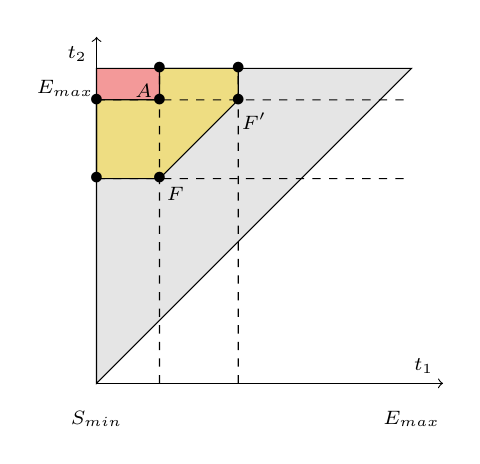
\begin{tikzpicture}
[scale=0.4]
\fill[gray!20] (0,0) -- (10,10) -- (0,10) -- cycle;
\draw[fill=LightCoral!80!] (0,10) rectangle (2,9);
\draw[fill=LightGoldenrod] (0,6.5) -- (2,6.5) -- (4.5,9) -- (4.5,10)
-- (2,10) -- (2,9) -- (0,9) -- cycle; 
\node (O) at (0,0) {};
\node (T1) at (11,0) {};
\node (T2) at (0,11) {};

\node at (0,0) {};
\node[label={[shift={(-0.4,-0.6)}]\scriptsize$\LE$}] (di) at (0,9) {$\bullet$};
\node[label={[shift={(-0.4,-0.6)}]\scriptsize$E_{max}$}] at (0,10) {};

\node[label={[shift={(0,-0.8)}]\scriptsize$S_{min}$}] at (0,0) {};
\node[label={[shift={(0,-0.8)}]\scriptsize$\ES$}] (ri) at (2,0) {};
\node[label={[shift={(0,-0.8)}]\scriptsize$E_{max}$}] at (10,0) {};
\node[label={[shift={(-0.4,-0.6)}]\scriptsize$\smax$}] (smax2) at (0,6.5) {$\bullet$};

\node[label={[shift={(0,-0.8)}]\scriptsize$\emin$}] (emin1) at (4.5,0) {};

\node at (2,10) {$\bullet$};
\node at (4.5,10) {$\bullet$};

\node at (2,3) {};
\node at (5,5) {};
\node[label={[shift={(-0.2,-0.3)}]\scriptsize$A$}] (A) at (2,9) {$\bullet$};
\node[label={[shift={(0.2,-0.6)}]\scriptsize$F$}] at (2,6.5) {$\bullet$};
\node[label={[shift={(0.2,-0.7)}]\scriptsize$F'$}] at (4.5,9) {$\bullet$};
\draw[dashed] (ri.center) -- (2,10);
\draw[dashed] (di.center) -- (10,9);
\path[draw] (O.center) -- (10,10) -- (0,10) -- cycle;
\draw[dashed] (emin1.center) -- (4.5,10);
\draw[dashed] (smax2.center) -- (10,6.5);

\draw[->] (O.center) -- (T1.center) node[above left] {\scriptsize$t_1$};
\draw[->] (O.center) -- (T2.center) node[below left] {\scriptsize$t_2$};
\end{tikzpicture}}

\vspace{0.7cm}
Cas $ W_i \le f_i(\bmin) (\LE-\ES)$


\subcaptionbox{$ \emin \le \smax $}[0.45\linewidth]{

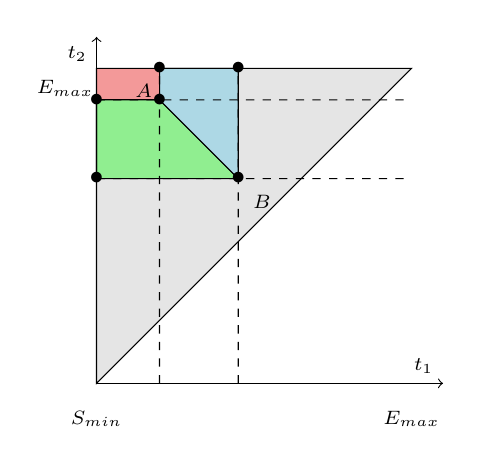
\begin{tikzpicture}
[scale=0.4]
%non common
\fill[gray!20] (0,0) -- (10,10) -- (0,10) -- cycle;
\draw[fill=LightGreen] (0,9) -- (2,9) -- (4.5,6.5) --(0,6.5) -- cycle;
\draw[fill=LightBlue] (2,9) -- (2,10) -- (4.5,10) --(4.5,6.5) --cycle;
\node[label={[shift={(0.3,-0.7)}]\scriptsize$B$}] (B) at (4.5,6.5) {$\bullet$};
\node[label={[shift={(-0.4,-0.6)}]\scriptsize$\smax$}] (smax2) at (0,6.5) {$\bullet$};

\node[label={[shift={(0,-0.8)}]\scriptsize$\emin$}] (emin1) at (4.5,0) {};
\node at (4.5,10) {$\bullet$};
%common

\draw[fill=LightCoral!80!] (0,10) rectangle (2,9);
\node (O) at (0,0) {};
\node (T1) at (11,0) {};
\node (T2) at (0,11) {};


\node[label={[shift={(-0.4,-0.6)}]\scriptsize$\LE$}] (di) at (0,9) {$\bullet$};
\node[label={[shift={(-0.4,-0.6)}]\scriptsize$E_{max}$}] at (0,10) {};

\node[label={[shift={(0,-0.8)}]\scriptsize$S_{min}$}] at (0,0) {};
\node[label={[shift={(0,-0.8)}]\scriptsize$\ES$}] (ri) at (2,0) {};
\node[label={[shift={(0,-0.8)}]\scriptsize$E_{max}$}] at (10,0) {};

\node at (2,10) {$\bullet$};

\node[label={[shift={(-0.2,-0.3)}]\scriptsize$A$}] (A) at (2,9) {$\bullet$};

\draw[dashed] (ri.center) -- (2,10);
\draw[dashed] (emin1.center) -- (4.5,10);
\draw[dashed] (di.center) -- (10,9);
\draw[dashed] (smax2.center) -- (10,6.5);
\path[draw] (O.center) -- (10,10) -- (0,10) -- cycle;
\draw[->] (O.center) -- (T1.center) node[above left] {\scriptsize$t_1$};
\draw[->] (O.center) -- (T2.center) node[below left] {\scriptsize$t_2$};
\end{tikzpicture}}
\hfill
\subcaptionbox{$\emin \ge \smax$}[0.45\linewidth]{
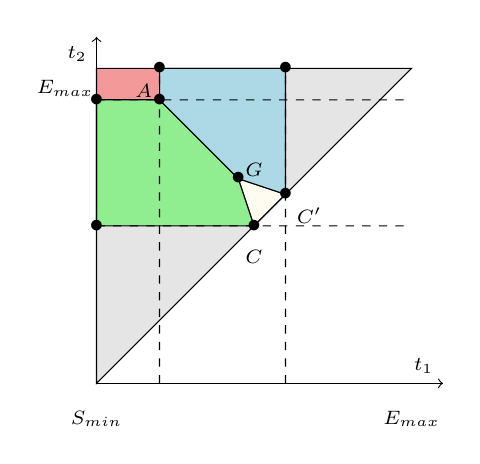
\begin{tikzpicture}
[scale=0.4]
\fill[gray!20] (0,0) -- (10,10) -- (0,10) -- cycle;
\draw[fill=Cornsilk!99!black!40!] (6,6) -- (5,5) -- (4.5,6.5) -- cycle;
\draw[fill=LightGreen] (0,9) -- (2,9)-- (4.5,6.5) -- (5,5) -- (0,5) -- cycle;
\draw[fill=LightBlue]  (2,9) -- (2,10)-- (6,10) -- (6,6)-- (4.5,6.5) -- cycle;
\node[label={[shift={(0,-0.8)}]\scriptsize$C$}] (C) at (5,5)  {$\bullet$};
\node[label={[shift={(0.3,-0.7)}]\scriptsize$C'$}] (C2) at (6,6)  {$\bullet$};

\node[label={[shift={(0.2,-0.3)}]\scriptsize$G$}] at (4.5,6.5)  {$\bullet$};
\node[label={[shift={(-0.4,-0.6)}]\scriptsize$\smax$}] (smax2) at (0,5) {$\bullet$};

\node[label={[shift={(0,-0.8)}]\scriptsize$\emin$}] (emin1) at (6,0) {};

\node at (6,10) {$\bullet$};
%common

\draw[fill=LightCoral!80!] (0,10) rectangle (2,9);
\node (O) at (0,0) {};
\node (T1) at (11,0) {};
\node (T2) at (0,11) {};

\node[label={[shift={(-0.4,-0.6)}]\scriptsize$\LE$}] (di) at (0,9) {$\bullet$};
\node[label={[shift={(-0.4,-0.6)}]\scriptsize$E_{max}$}] at (0,10) {};

\node[label={[shift={(0,-0.8)}]\scriptsize$S_{min}$}] at (0,0) {};
\node[label={[shift={(0,-0.8)}]\scriptsize$\ES$}] (ri) at (2,0) {};
\node[label={[shift={(0,-0.8)}]\scriptsize$E_{max}$}] at (10,0) {};

\node at (2,10) {$\bullet$};

\node at (2,3) {};
\node at (5,5) {};
\node[label={[shift={(-0.2,-0.3)}]\scriptsize$A$}] (A) at (2,9) {$\bullet$};

\draw[dashed] (ri.center) -- (2,10);
\draw[dashed] (emin1.center) -- (6,10);
\draw[dashed] (di.center) -- (10,9);
\draw[dashed] (smax2.center) -- (10,5);
\path[draw] (O.center) -- (10,10) -- (0,10) -- cycle;
\draw[->] (O.center) -- (T1.center) node[above left] {\scriptsize$t_1$};
\draw[->] (O.center) -- (T2.center) node[below left] {\scriptsize$t_2$};

\end{tikzpicture}
}

\vspace{0.7cm}
Cas $  W_i \ge f_i(\bmin) (\LE - \ES)$

\subcaptionbox{$\emin \le \smax$}[0.45\linewidth]{

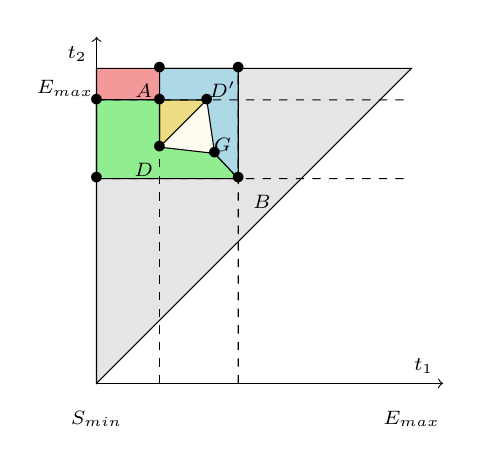
\begin{tikzpicture}
[scale=0.4]
%non common

\fill[gray!20] (0,0) -- (10,10) -- (0,10) -- cycle;
\path[fill=Cornsilk!99!black!40!] (2,7.5) -- (3.5,9)-- (3.75,7.3) -- cycle;
\draw[fill=LightGoldenrod] (2,7.5) -- (3.5,9) -- (2,9) -- cycle;
\draw[fill=LightGreen] (0,9) -- (2,9) -- (2,7.5)  --  (3.75,7.3) -- (4.5,6.5) -- (0,6.5)  -- (0,7.5) --cycle;
%\draw[fill=PaleGreen!70!] (0,7.5) -- (2,7.5) -- (3.75,7.3) --
%(4.5,6.5) -- (0,6.5) -- cycle;
\draw[fill=LightBlue] (2,9) -- (2,10) -- (4.5,10) --  (4.5,6.5) --
(3.75,7.3) -- (3.5,9) -- cycle;
%\draw[fill=PowderBlue!70!] (4.5,6.5)-- (3.75,7.3) -- (3.5,9) -- (3.5,10) -- (4.5,10) --cycle;
\node[label={[shift={(-0.2,-0.7)}]\scriptsize$D$}] (D) at (2,7.5) {$\bullet$};
\node[label={[shift={(0.2,-0.3)}]\scriptsize$D'$}] (D2) at (3.5,9) {$\bullet$};
\node[label={[shift={(0.1,-0.3)}]\scriptsize$G$}] (E) at (3.75,7.3)  {$\bullet$};
\node[label={[shift={(0.3,-0.7)}]\scriptsize$B$}] (B) at (4.5,6.5) {$\bullet$};
\node[label={[shift={(-0.4,-0.6)}]\scriptsize$\smax$}] (smax2) at (0,6.5) {$\bullet$};

\node[label={[shift={(0,-0.8)}]\scriptsize$\emin$}] (emin1) at (4.5,0) {};
\node at (4.5,10) {$\bullet$};
%\node at (3.5,10) {$\bullet$};
%\node at (0,7.5) {$\bullet$};
%common


\draw[fill=LightCoral!80!] (0,10) rectangle (2,9);
\node (O) at (0,0) {};
\node (T1) at (11,0) {};
\node (T2) at (0,11) {};


\node[label={[shift={(-0.4,-0.6)}]\scriptsize$\LE$}] (di) at (0,9) {$\bullet$};
\node[label={[shift={(-0.4,-0.6)}]\scriptsize$E_{max}$}] at (0,10) {};

\node[label={[shift={(0,-0.8)}]\scriptsize$S_{min}$}] at (0,0) {};
\node[label={[shift={(0,-0.8)}]\scriptsize$\ES$}] (ri) at (2,0) {};
\node[label={[shift={(0,-0.8)}]\scriptsize$E_{max}$}] at (10,0) {};

\node at (2,10) {$\bullet$};

\node at (2,3) {};
\node at (5,5) {};
\node[label={[shift={(-0.2,-0.3)}]\scriptsize$A$}] (A) at (2,9) {$\bullet$};

\draw[dashed] (ri.center) -- (D.center);
\draw[dashed] (emin1.center) -- (4.5,10);
\draw[dashed] (di.center) -- (10,9);
\draw[dashed] (smax2.center) -- (10,6.5);
\path[draw] (O.center) -- (10,10) -- (0,10) -- cycle;
\draw[->] (O.center) -- (T1.center) node[above left] {\scriptsize$t_1$};
\draw[->] (O.center) -- (T2.center) node[below left] {\scriptsize$t_2$};

\end{tikzpicture}
}
\hfill
\subcaptionbox{$\emin \ge \smax$}[0.45\linewidth]{

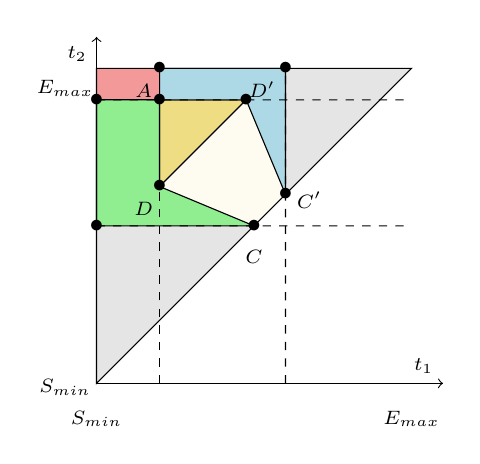
\begin{tikzpicture}
[scale=0.4]
%non common

\fill[gray!20] (0,0) -- (10,10) -- (0,10) -- cycle;
\path[fill=Cornsilk!99!black!40!] (2,6.25) -- (4.75,9)-- (6,6) -- (5,5) -- cycle;
\draw[fill=LightGoldenrod] (2,6.25) -- (2,9) -- (4.75,9) -- cycle;
\draw[fill=LightGreen] (0,9) -- (2,9) -- (2,6.25) --  (5,5)
-- (0,5) --  cycle;
%\draw[fill=PaleGreen!70!] (0,6.25) -- (2,6.25) -- (5,5) -- (0,5) -- cycle;
\draw[fill=LightBlue] (2,9) -- (2,10) -- (4.75,10) -- (6,10) -- (6,6) -- (4.75,9) -- cycle;
%\draw[fill=PowderBlue!70!] (4.75,10) -- (6,10) -- (6,6)-- (4.75,9) -- cycle;
\node[label={[shift={(-0.2,-0.7)}]\scriptsize$D$}] (D) at (2,6.25) {$\bullet$};
\node[label={[shift={(0.2,-0.3)}]\scriptsize$D'$}] (D2) at (4.75,9) {$\bullet$};
\node[label={[shift={(0,-0.8)}]\scriptsize$C$}] (C) at (5,5)  {$\bullet$};
\node[label={[shift={(0.3,-0.5)}]\scriptsize$C'$}] (C2) at (6,6)  {$\bullet$};
\node[label={[shift={(-0.4,-0.6)}]\scriptsize$\smax$}] (smax2) at (0,5) {$\bullet$};

\node[label={[shift={(0,-0.8)}]\scriptsize$\emin$}] (emin1) at (6,0) {};

\node at (6,10) {$\bullet$};
%\node at (4.75,10) {$\bullet$};
%\node at (0,6.25) {$\bullet$};
%common

\draw[fill=LightCoral!80!] (0,10) rectangle (2,9);
\node (O) at (0,0) {};
\node (T1) at (11,0) {};
\node (T2) at (0,11) {};

\node[label={[shift={(-0.4,-0.4)}]\scriptsize$S_{min}$}] at (0,0) {};
\node[label={[shift={(-0.4,-0.6)}]\scriptsize$\LE$}] (di) at (0,9) {$\bullet$};
\node[label={[shift={(-0.4,-0.6)}]\scriptsize$E_{max}$}] at (0,10) {};

\node[label={[shift={(0,-0.8)}]\scriptsize$S_{min}$}] at (0,0) {};
\node[label={[shift={(0,-0.8)}]\scriptsize$\ES$}] (ri) at (2,0) {};
\node[label={[shift={(0,-0.8)}]\scriptsize$E_{max}$}] at (10,0) {};

\node at (2,10) {$\bullet$};

\node at (2,3) {};
\node at (5,5) {};
\node[label={[shift={(-0.2,-0.3)}]\scriptsize$A$}] (A) at (2,9) {$\bullet$};

\draw[dashed] (ri.center) -- (D.center);
\draw[dashed] (emin1.center) -- (6,10);
\draw[dashed] (di.center) -- (10,9);
\draw[dashed] (smax2.center) -- (10,5);
\path[draw] (O.center) -- (10,10) -- (0,10) -- cycle;
\draw[->] (O.center) -- (T1.center) node[above left] {\scriptsize$t_1$};
\draw[->] (O.center) -- (T2.center) node[below left] {\scriptsize$t_2$};

\end{tikzpicture}

}
\caption{Les différentes expressions de $\wb$ en fonction des
  paramètres du problème \CECSP.}
\label{fig:breakline_nrj}
\end{figure}

Nous avons donc défini les différentes zones correspondant chacune à
une expression de $\wb$. Dans le cas où, $f_i$ est la fonction
identité, cela suffit pour définir les segments à considérer, i.e. les
segments pour lesquels on va tester l'intersection. La méthode
générale pour calculer les intervalles d'intérêt en fonction de ces
segments sera détaillée un peu plus loin dans le paragraphe. 

Les segments à considérer sont les segments délimitant deux zones avec
une expression de $\wb$ différentes, i.e. reliant deux points
représentés par une boule noire sur la
figure~\ref{fig:breakline_nrj}. Par exemple, dans le cas où $W_i \ge
f_i(\bmin)(\LE-\ES)$ les segments à considérer sont donc:
\begin{itemize}
\item dans le cas $\emin \le \smax$: $(\ES ,E_{max})A,\ (S_{min},
\LE)A,\ (S_{min},\smax)B,\ B(\emin,E_{max}),\ AD,\ AD',\
DD' ,\ DG,\ D'G$ and $GB$.
\item for case $\emin\ge \smax$: $(\ES ,E_{max})A,\ (S_{min},
\LE)A,\ (S_{min},\smax)C,\ C'(\emin,E_{max}),\ AD,\ AD',\
DD' ,\ DC$ and $D'C$.
\end{itemize}
avec $D_{t_1}$ (resp. $D_{t_2}$) la projection sur l'axe $x$
(resp. sur l'axe $y$) du point $D$.


Nous allons maintenant calculer, à partir de la
figure~\ref{fig:breakline_nrj}, les zones correspondant à des
expressions différentes de $\bb$. 

Pour ce faire, nous considérons, à l'intérieur de chaque zone définie
pour $\wb$, l'inégalité suivante: 
\[ \frac{\wb}{f_i(\bmin)} \le |I|\]
avec $I=[t_1,t_2[ \cap [\ES,\LE]$. Si cette condition est vérifiée,
alors l'activité peut être ordonnancée à $\bmin$ et l'expression de
$\bb$ sera alors $\frac{\wb}{f_i(\bmin)}\times \bmin$. Dans le cas
inverse, nous avons $\bb=\frac{1}{a_i}(\wb-c_i|I|)$. 

Dans le cas $\bmin=0$, l'inégalité n'a pas besoin d'être considérée et
nous avons directement $\bb=\frac{1}{a_i}(\wb-c_i|I|)$ dans chaque
zone. 

Dans le cas où $W_i\le f_i(\bmin)(\LE-\ES)$, $|I|$ peut valoir
$t_2-t_1$, $t_2-\ES$, $\LE-t_1$ ou $\LE-\ES$. 

Dans le premier cas,
l'inégalité donne $\wb \le f_i(\bmin)(t_2-t_1)$. Or, ce cas correspond
au cas où $[t_1,t_2[ \subset [\ES,\LE]$ et donc, $\wb=\min(W_i -
f_i(\bmax)(\LE-t_2), W_i - f_i(\bmax)(t_1-\ES),
f_i(\bmin)(t_2-t_1))$. Donc, dans ce cas, l'inégalité est toujours
vérifiée et nous avons $\bb = \bmin \times \wb/f_i(\bmin)$ dans le cas
où $[t_1,t_2[ \subset [\ES,\LE]$. 

Dans le second cas,
i.e. $|I|=t_2-\ES$, l'inégalité donne $\wb \le
f_i(\bmin)(t_2-\ES)$. Or, ce cas correspond au cas où $\wb = W_i -
f_i(\bmax)(\LE -t_2)$ , i.e. la zone verte. En remplaçant $\wb$ par
son expression, nous obtenons l'inégalité suivante: 
\[t_2 \le \frac{f_i(\bmax)\LE - f_i(\bmin)\ES - W_i }{f_i(\bmax) -
    f_i(\bmin)} \]
Or, $\LE  \le \frac{f_i(\bmax)\LE - f_i(\bmin)\ES - W_i }{f_i(\bmax) -
  f_i(\bmin)}$. Donc, nous l'inégalité est vérifiée si $t_2 \le d_i$
et ceci est vrai dans ce cas. 

Les cas où $|I| = \LE -\ES$ et $|I| =
\LE -t_1$ sont traités de la même façon. Donc, dans le cas où $W_i \le
f_i(\bmin) (\LE - \ES)$, $\bb=\bmin \times \wb/f_i(\bmin)$ et les
zones où $\bb$ a la même expression sont les mêmes que pour $\wb$ dans
ce cas. 



\begin{figure}[!htb]
  \centering
   \subcaptionbox{Cas $\bmin = 0$}[0.45\linewidth]
{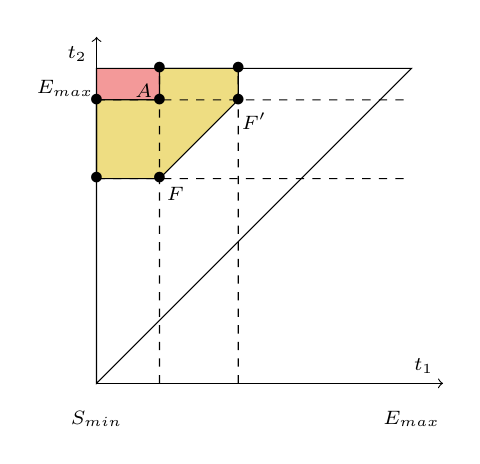
\begin{tikzpicture}
[scale=0.4]
\draw[fill=LightCoral!80!] (0,10) rectangle (2,9);
\draw[fill=LightGoldenrod] (0,6.5) -- (2,6.5) -- (4.5,9) -- (4.5,10) -- (2,10) -- (2,9) -- (0,9) -- cycle;
\node (O) at (0,0) {};
\node (T1) at (11,0) {};
\node (T2) at (0,11) {};

\node at (0,0) {};
\node[label={[shift={(-0.4,-0.6)}]\scriptsize$\LE$}] (di) at (0,9) {$\bullet$};
\node[label={[shift={(-0.4,-0.6)}]\scriptsize$E_{max}$}] at (0,10) {};

\node[label={[shift={(0,-0.8)}]\scriptsize$S_{min}$}] at (0,0) {};
\node[label={[shift={(0,-0.8)}]\scriptsize$\ES$}] (ri) at (2,0) {};
\node[label={[shift={(0,-0.8)}]\scriptsize$E_{max}$}] at (10,0) {};
\node[label={[shift={(-0.4,-0.6)}]\scriptsize$\smax$}] (smax2) at (0,6.5) {$\bullet$};

\node[label={[shift={(0,-0.8)}]\scriptsize$\emin$}] (emin1) at (4.5,0) {};

\node at (2,10) {$\bullet$};
\node at (4.5,10) {$\bullet$};

\node at (2,3) {};
\node at (5,5) {};
\node[label={[shift={(-0.2,-0.3)}]\scriptsize$A$}] (A) at (2,9) {$\bullet$};
\node[label={[shift={(0.2,-0.6)}]\scriptsize$F$}] at (2,6.5) {$\bullet$};
\node[label={[shift={(0.2,-0.7)}]\scriptsize$F'$}] at (4.5,9) {$\bullet$};
\draw[dashed] (ri.center) -- (2,10);
\draw[dashed] (di.center) -- (10,9);
\path[draw] (O.center) -- (10,10) -- (0,10) -- cycle;
\draw[dashed] (emin1.center) -- (4.5,10);
\draw[dashed] (smax2.center) -- (10,6.5);

\draw[->] (O.center) -- (T1.center) node[above left] {\scriptsize$t_1$};
\draw[->] (O.center) -- (T2.center) node[below left] {\scriptsize$t_2$};
\end{tikzpicture}}

\vspace{0.7cm}
Cas $ W_i \le f_i(\bmin) (\LE-\ES)$


\subcaptionbox{$ \emin \le \smax $}[0.45\linewidth]{

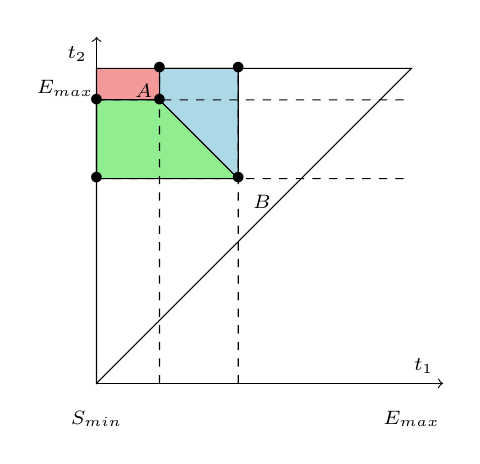
\begin{tikzpicture}
[scale=0.4]
%non common
\draw[fill=LightGreen] (0,9) -- (2,9) -- (4.5,6.5) --(0,6.5) -- cycle;
\draw[fill=LightBlue] (2,9) -- (2,10) -- (4.5,10) --(4.5,6.5) --cycle;
\node[label={[shift={(0.3,-0.7)}]\scriptsize$B$}] (B) at (4.5,6.5) {$\bullet$};
\node[label={[shift={(-0.4,-0.6)}]\scriptsize$\smax$}] (smax2) at (0,6.5) {$\bullet$};

\node[label={[shift={(0,-0.8)}]\scriptsize$\emin$}] (emin1) at (4.5,0) {};
\node at (4.5,10) {$\bullet$};
%common

\draw[fill=LightCoral!80!] (0,10) rectangle (2,9);
\node (O) at (0,0) {};
\node (T1) at (11,0) {};
\node (T2) at (0,11) {};


\node[label={[shift={(-0.4,-0.6)}]\scriptsize$\LE$}] (di) at (0,9) {$\bullet$};
\node[label={[shift={(-0.4,-0.6)}]\scriptsize$E_{max}$}] at (0,10) {};

\node[label={[shift={(0,-0.8)}]\scriptsize$S_{min}$}] at (0,0) {};
\node[label={[shift={(0,-0.8)}]\scriptsize$\ES$}] (ri) at (2,0) {};
\node[label={[shift={(0,-0.8)}]\scriptsize$E_{max}$}] at (10,0) {};

\node at (2,10) {$\bullet$};

\node[label={[shift={(-0.2,-0.3)}]\scriptsize$A$}] (A) at (2,9) {$\bullet$};

\draw[dashed] (ri.center) -- (2,10);
\draw[dashed] (emin1.center) -- (4.5,10);
\draw[dashed] (di.center) -- (10,9);
\draw[dashed] (smax2.center) -- (10,6.5);
\path[draw] (O.center) -- (10,10) -- (0,10) -- cycle;
\draw[->] (O.center) -- (T1.center) node[above left] {\scriptsize$t_1$};
\draw[->] (O.center) -- (T2.center) node[below left] {\scriptsize$t_2$};
\end{tikzpicture}}
\hfill
\subcaptionbox{$\emin \ge \smax$}[0.45\linewidth]{
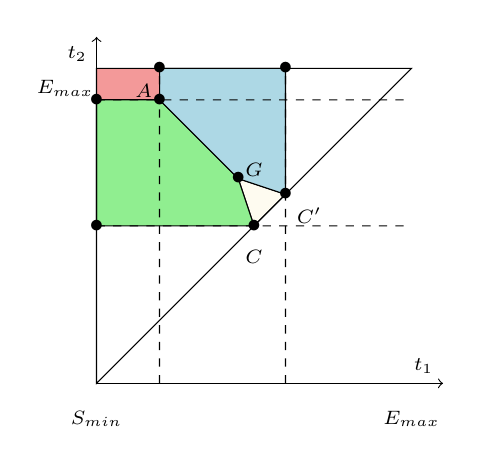
\begin{tikzpicture}
[scale=0.4]
\draw[fill=Cornsilk!99!black!40!] (6,6) -- (5,5) -- (4.5,6.5) -- cycle;
\draw[fill=LightGreen] (0,9) -- (2,9)-- (4.5,6.5) -- (5,5) -- (0,5) -- cycle;
\draw[fill=LightBlue]  (2,9) -- (2,10)-- (6,10) -- (6,6)-- (4.5,6.5) -- cycle;
\node[label={[shift={(0,-0.8)}]\scriptsize$C$}] (C) at (5,5)  {$\bullet$};
\node[label={[shift={(0.3,-0.7)}]\scriptsize$C'$}] (C2) at (6,6)  {$\bullet$};

\node[label={[shift={(0.2,-0.3)}]\scriptsize$G$}] at (4.5,6.5)  {$\bullet$};
\node[label={[shift={(-0.4,-0.6)}]\scriptsize$\smax$}] (smax2) at (0,5) {$\bullet$};

\node[label={[shift={(0,-0.8)}]\scriptsize$\emin$}] (emin1) at (6,0) {};

\node at (6,10) {$\bullet$};
%common

\draw[fill=LightCoral!80!] (0,10) rectangle (2,9);
\node (O) at (0,0) {};
\node (T1) at (11,0) {};
\node (T2) at (0,11) {};

\node[label={[shift={(-0.4,-0.6)}]\scriptsize$\LE$}] (di) at (0,9) {$\bullet$};
\node[label={[shift={(-0.4,-0.6)}]\scriptsize$E_{max}$}] at (0,10) {};

\node[label={[shift={(0,-0.8)}]\scriptsize$S_{min}$}] at (0,0) {};
\node[label={[shift={(0,-0.8)}]\scriptsize$\ES$}] (ri) at (2,0) {};
\node[label={[shift={(0,-0.8)}]\scriptsize$E_{max}$}] at (10,0) {};

\node at (2,10) {$\bullet$};

\node at (2,3) {};
\node at (5,5) {};
\node[label={[shift={(-0.2,-0.3)}]\scriptsize$A$}] (A) at (2,9) {$\bullet$};

\draw[dashed] (ri.center) -- (2,10);
\draw[dashed] (emin1.center) -- (6,10);
\draw[dashed] (di.center) -- (10,9);
\draw[dashed] (smax2.center) -- (10,5);
\path[draw] (O.center) -- (10,10) -- (0,10) -- cycle;
\draw[->] (O.center) -- (T1.center) node[above left] {\scriptsize$t_1$};
\draw[->] (O.center) -- (T2.center) node[below left] {\scriptsize$t_2$};

\end{tikzpicture}
}

\vspace{0.7cm}
Cas $  W_i \ge f_i(\bmin) (\LE - \ES)$

\subcaptionbox{$\emin \le \smax$}[0.45\linewidth]{

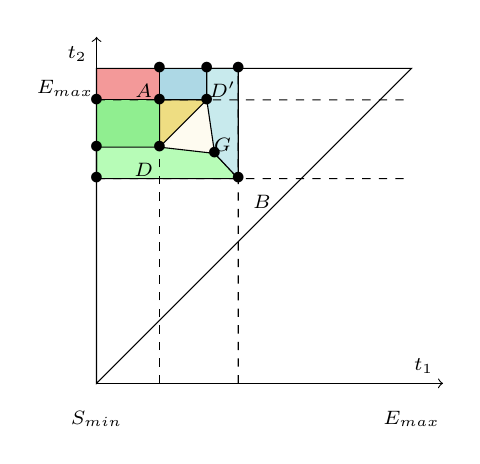
\begin{tikzpicture}
[scale=0.4]
%non common
\path[fill=Cornsilk!99!black!40!] (2,7.5) -- (3.5,9)-- (3.75,7.3) -- cycle;
\draw[fill=LightGoldenrod] (2,7.5) -- (3.5,9) -- (2,9) -- cycle;
\draw[fill=LightGreen] (0,9) -- (2,9) -- (2,7.5) -- (0,7.5) --cycle;
\draw[fill=PaleGreen!70!] (0,7.5) -- (2,7.5) -- (3.75,7.3) -- (4.5,6.5) -- (0,6.5) -- cycle;
\draw[fill=LightBlue] (2,9) -- (2,10) -- (3.5,10) --(3.5,9)--cycle;
\draw[fill=PowderBlue!70!] (4.5,6.5)-- (3.75,7.3) -- (3.5,9) -- (3.5,10) -- (4.5,10) --cycle;
\node[label={[shift={(-0.2,-0.7)}]\scriptsize$D$}] (D) at (2,7.5) {$\bullet$};
\node[label={[shift={(0.2,-0.3)}]\scriptsize$D'$}] (D2) at (3.5,9) {$\bullet$};
\node[label={[shift={(0.1,-0.3)}]\scriptsize$G$}] (E) at (3.75,7.3)  {$\bullet$};
\node[label={[shift={(0.3,-0.7)}]\scriptsize$B$}] (B) at (4.5,6.5) {$\bullet$};
\node[label={[shift={(-0.4,-0.6)}]\scriptsize$\smax$}] (smax2) at (0,6.5) {$\bullet$};

\node[label={[shift={(0,-0.8)}]\scriptsize$\emin$}] (emin1) at (4.5,0) {};
\node at (4.5,10) {$\bullet$};
\node at (3.5,10) {$\bullet$};
\node at (0,7.5) {$\bullet$};
%common

\draw[fill=LightCoral!80!] (0,10) rectangle (2,9);
\node (O) at (0,0) {};
\node (T1) at (11,0) {};
\node (T2) at (0,11) {};


\node[label={[shift={(-0.4,-0.6)}]\scriptsize$\LE$}] (di) at (0,9) {$\bullet$};
\node[label={[shift={(-0.4,-0.6)}]\scriptsize$E_{max}$}] at (0,10) {};

\node[label={[shift={(0,-0.8)}]\scriptsize$S_{min}$}] at (0,0) {};
\node[label={[shift={(0,-0.8)}]\scriptsize$\ES$}] (ri) at (2,0) {};
\node[label={[shift={(0,-0.8)}]\scriptsize$E_{max}$}] at (10,0) {};

\node at (2,10) {$\bullet$};

\node at (2,3) {};
\node at (5,5) {};
\node[label={[shift={(-0.2,-0.3)}]\scriptsize$A$}] (A) at (2,9) {$\bullet$};

\draw[dashed] (ri.center) -- (D.center);
\draw[dashed] (emin1.center) -- (4.5,10);
\draw[dashed] (di.center) -- (10,9);
\draw[dashed] (smax2.center) -- (10,6.5);
\path[draw] (O.center) -- (10,10) -- (0,10) -- cycle;
\draw[->] (O.center) -- (T1.center) node[above left] {\scriptsize$t_1$};
\draw[->] (O.center) -- (T2.center) node[below left] {\scriptsize$t_2$};

\end{tikzpicture}
}
\hfill
\subcaptionbox{$\emin \ge \smax$}[0.45\linewidth]{

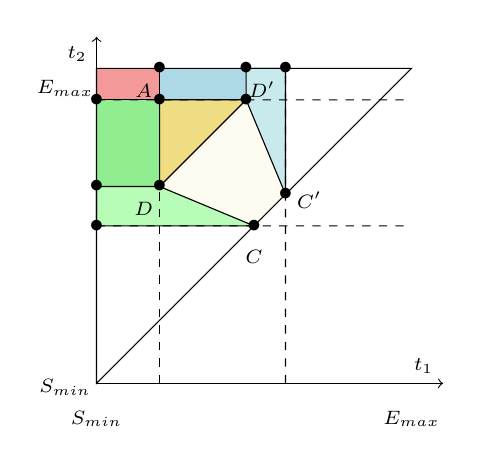
\begin{tikzpicture}
[scale=0.4]
%non common
\path[fill=Cornsilk!99!black!40!] (2,6.25) -- (4.75,9)-- (6,6) -- (5,5) -- cycle;
\draw[fill=LightGoldenrod] (2,6.25) -- (2,9) -- (4.75,9) -- cycle;
\draw[fill=LightGreen] (0,9) -- (2,9) -- (2,6.25) -- (0,6.25) -- cycle;
\draw[fill=PaleGreen!70!] (0,6.25) -- (2,6.25) -- (5,5) -- (0,5) -- cycle;
\draw[fill=LightBlue] (2,9) -- (2,10) -- (4.75,10) -- (4.75,9) -- cycle;
\draw[fill=PowderBlue!70!] (4.75,10) -- (6,10) -- (6,6)-- (4.75,9) -- cycle;
\node[label={[shift={(-0.2,-0.7)}]\scriptsize$D$}] (D) at (2,6.25) {$\bullet$};
\node[label={[shift={(0.2,-0.3)}]\scriptsize$D'$}] (D2) at (4.75,9) {$\bullet$};
\node[label={[shift={(0,-0.8)}]\scriptsize$C$}] (C) at (5,5)  {$\bullet$};
\node[label={[shift={(0.3,-0.5)}]\scriptsize$C'$}] (C2) at (6,6)  {$\bullet$};
\node[label={[shift={(-0.4,-0.6)}]\scriptsize$\smax$}] (smax2) at (0,5) {$\bullet$};

\node[label={[shift={(0,-0.8)}]\scriptsize$\emin$}] (emin1) at (6,0) {};

\node at (6,10) {$\bullet$};
\node at (4.75,10) {$\bullet$};
\node at (0,6.25) {$\bullet$};
%common

\draw[fill=LightCoral!80!] (0,10) rectangle (2,9);
\node (O) at (0,0) {};
\node (T1) at (11,0) {};
\node (T2) at (0,11) {};

\node[label={[shift={(-0.4,-0.4)}]\scriptsize$S_{min}$}] at (0,0) {};
\node[label={[shift={(-0.4,-0.6)}]\scriptsize$\LE$}] (di) at (0,9) {$\bullet$};
\node[label={[shift={(-0.4,-0.6)}]\scriptsize$E_{max}$}] at (0,10) {};

\node[label={[shift={(0,-0.8)}]\scriptsize$S_{min}$}] at (0,0) {};
\node[label={[shift={(0,-0.8)}]\scriptsize$\ES$}] (ri) at (2,0) {};
\node[label={[shift={(0,-0.8)}]\scriptsize$E_{max}$}] at (10,0) {};

\node at (2,10) {$\bullet$};

\node at (2,3) {};
\node at (5,5) {};
\node[label={[shift={(-0.2,-0.3)}]\scriptsize$A$}] (A) at (2,9) {$\bullet$};

\draw[dashed] (ri.center) -- (D.center);
\draw[dashed] (emin1.center) -- (6,10);
\draw[dashed] (di.center) -- (10,9);
\draw[dashed] (smax2.center) -- (10,5);
\path[draw] (O.center) -- (10,10) -- (0,10) -- cycle;
\draw[->] (O.center) -- (T1.center) node[above left] {\scriptsize$t_1$};
\draw[->] (O.center) -- (T2.center) node[below left] {\scriptsize$t_2$};

\end{tikzpicture}

}
\caption{Les différentes expressions de $\bb$ en fonction des
  paramètres du problème \CECSP.}
\label{fig:breakline_res}
\end{figure}
\subsubsection{Intervalles d'intérêt pour les ajustements}
